\chapter{手法}


\section{第一原理計算}
第一原理計算とは, シュレディンガー方程式を精確に解いて, 原子の種類だけから電子構造を求め, 様々な物性を予測する計算である. しかし, 第一原理計算は非常に高い精度が要求される複雑なものである.


\section{VASP}
VASP (Vienna Ab-initio Simulation Package) は, 密度汎関数理論による平面波・擬ポテンシャル法を用いた第一原理計算プログラムパッケージである. 密度汎関数理論とは電子系等のエネルギーなどの物性は電子密度から計算できるという理論である. 擬ポテンシャル法とは原子の内殻電子を除いた価電子だけを考慮する手法であり, 全電子を計算するフルポテンシャル法に比べ比較的高速な計算が可能となるため, 擬ポテンシャル法であっても十分な精度で計算ができる.
VASP の計算には, 計算条件が記述された INCAR, 計算モデルの構造が記述された POSCAR, 原子情報が記述された POTCAR, 計算精度を司る k−mesh が記述された KPOINTS の 4 種類の入力ファイルを使用し計算を行う. その後, 計算モデル内における原子の安定位置やフォース, 系の全体エネルギー等が記述された OUTCAR 等を出力する.


\section{計算モデル}
\subsection{周期的境界条件}
VASP で計算を行う場合, 平面波を用いた第一原理計算が行われるため, 無限周期の固体を考えなければならないが計算モデル内の原子が増えるにつれ計算時間も増えるため, 無限周期のモデルの計算を行うことはできない. そこで図 2.1 のように同じモデルが全方向に無限に隣接したようなモデルを考える. このモデルであれば, 無限周期の固体と見なせるため平面波を考慮することができる. このような計算条件を周期的境界条件という.

\begin{figure}[htbp]
	\begin{center}
		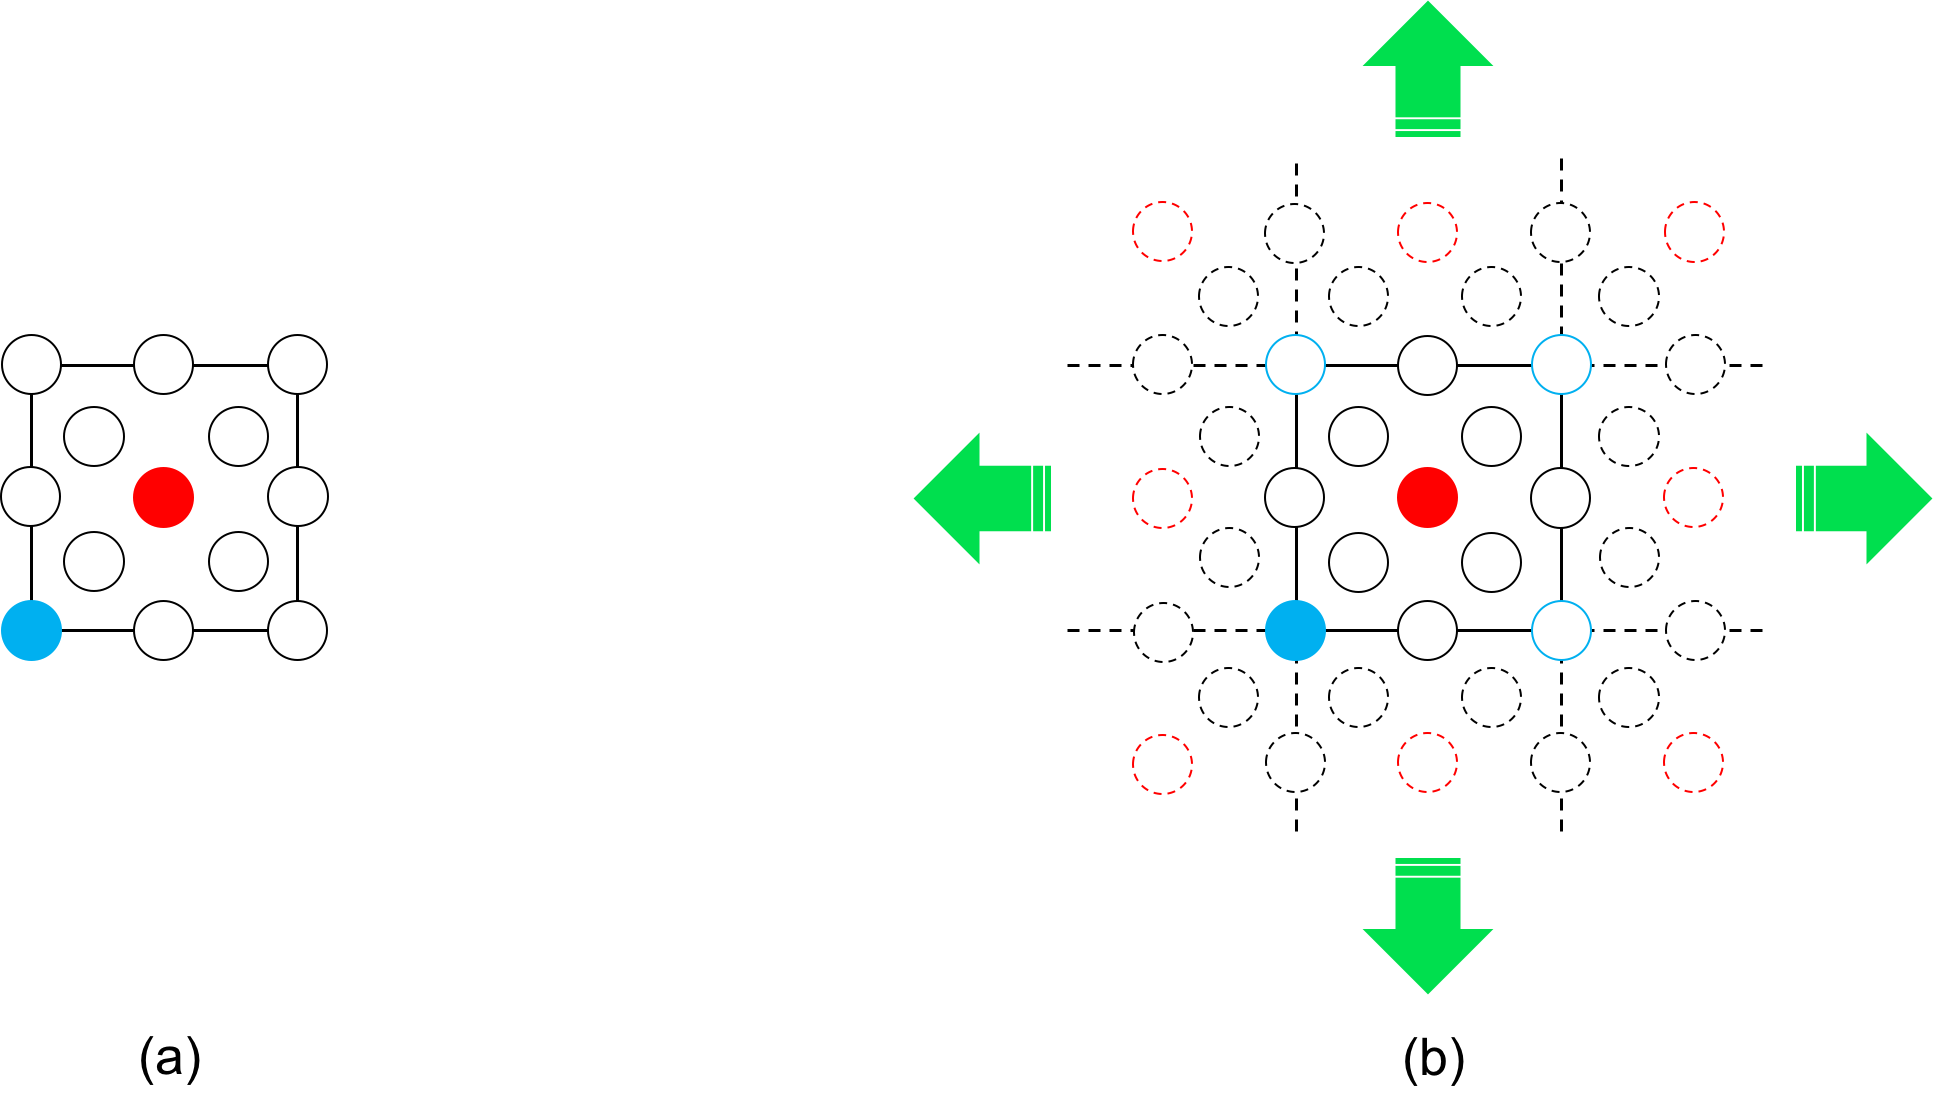
\includegraphics[width=130mm]{../method/cnd.png}
		\caption{(a) 周期的境界条件を考慮しないモデルの模式図.(b) 周期的境界条件を考慮したモデルの模式図.実線部分は計算モデル,破線部分は隣接した計算モデルを表している.}
		\label{default}
	\end{center}
\end{figure}


\subsection{ L1$_2$ クラスターおよび Small Cluster の導入}
清原らは,L12 クラスターを hcp 構造に強引に導入すると, 図2.2の (a), (b) のように縦方向と横方向の 2 つに分裂した集団が生成すると予測している\cite{kiyohara}. このサイズは実験的には奥田らが報告しているクラスターサイズに近い\cite{okuda}. 

\begin{figure}[htbp]
	\begin{center}
		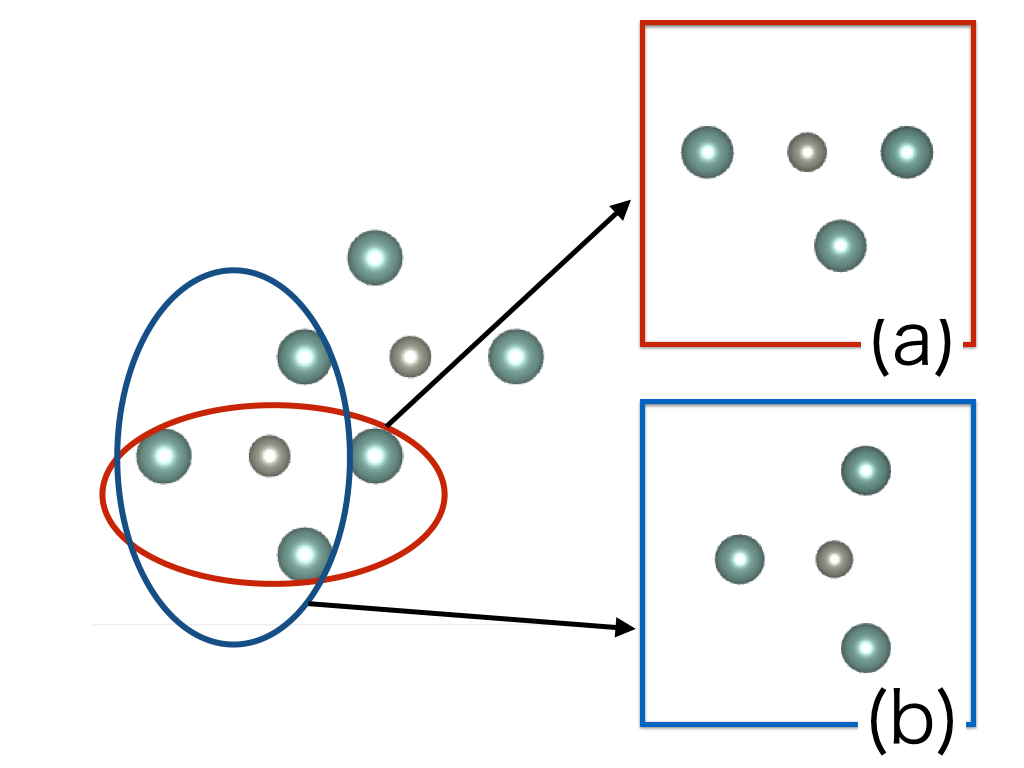
\includegraphics[width=50mm]{../method/MiniCluster.png}
		\caption{Small Cluster の模式図.}
		\label{default}
	\end{center}
\end{figure}

これらの集団を 6層の Mg 結晶に導入したモデルについて検証した. 系全体のエネルギーを第一原理計算により求めた結果, (a) のモデルが安定であるという結果が得られた. 今回, 本研究では (a) を Small Cluster とした. 西谷研究室では, Small Cluster と L1$_2$ クラスターの相互作用の計算モデルは, 必要最小の原子数でしか行っていなかった. そのため, Small Cluster も周期的に並んだモデルとなっている. より現実的なモデルとしては, 隣接する Small Cluster との相互作用の影響が及ばないだけの距離をとるサイズで計算する必要がある. そこで, 24層の slub モデルを構築し, Small Cluster を図 2.3 のように L1$_2$ クラスターから Small Cluster を1層ずつ離した slab モデルに挿入して, VASP を用いて第一原理計算を行い, 構造緩和したエネルギーを求めた.

\begin{figure}[htbp]
	\begin{center}
		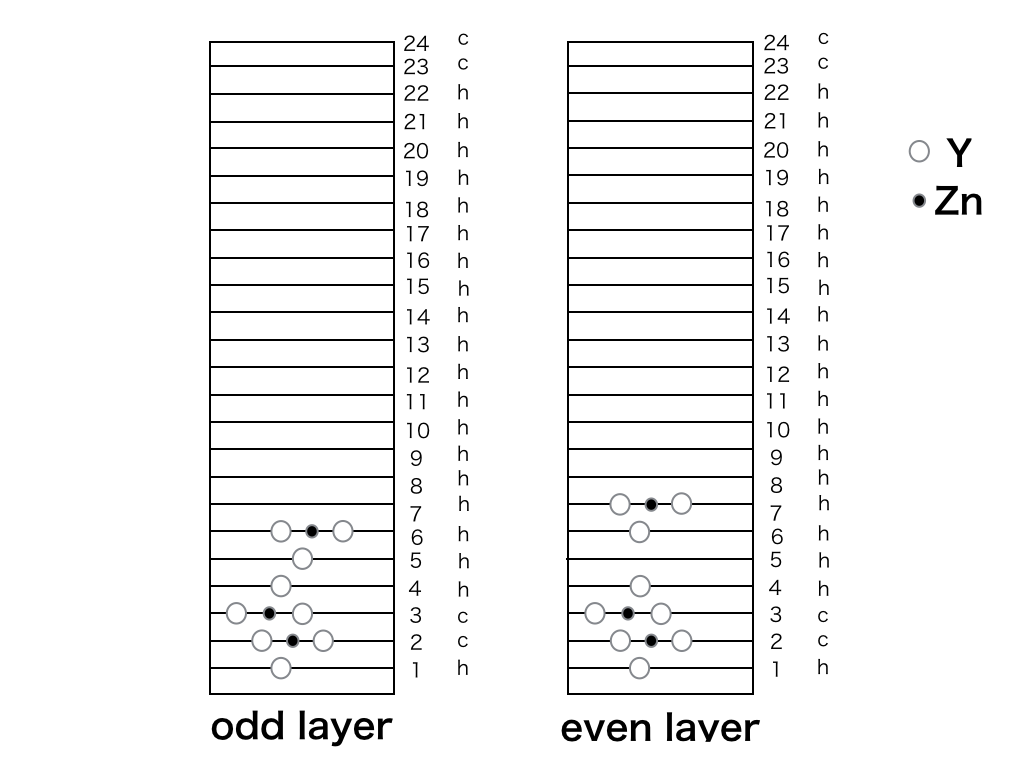
\includegraphics[width=80mm]{../method/small_cluster_slab.png}
		\caption{slub モデルの模式図.}
		\label{default}
	\end{center}
\end{figure}


\subsection{ Small Cluster および 空孔の導入}


\section{Small Cluster と空孔の挿入位置}
L1$_2$ クラスターを導入したモデルに Small Cluster や空孔を挿入するには様々な配置パターンがあり, すべての配置を考慮するのは困難である. そこで, 西谷研究室では, 各配置 場所に a から順に番号を振り分ける方法を用い, 各層での配置パターンを決定した. L1$_2$ クラスターから 1, 3, 5 …層離れた層は C 層, 2, 4 …層離れた層は A 層の配置となっている. アルファベットの組み合わせの模式図を図 2.4 で示した. また, 赤, 青, 緑, 黄丸はそれぞれ L1$_2$ クラスターから第 0~3 近接原子を表している.

\begin{figure}[htbp]
    \begin{tabular}{cc}
      \begin{minipage}{0.5\hsize}
        \centering
        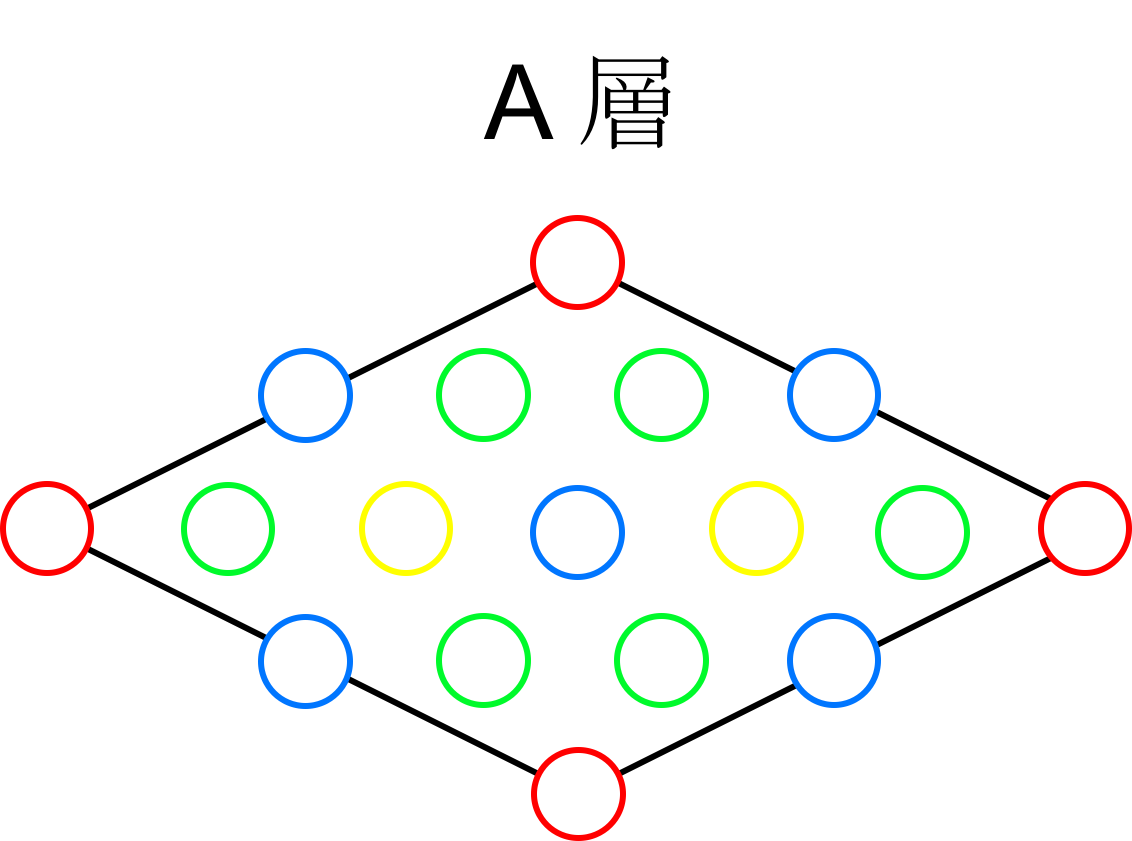
\includegraphics[width=80mm]{../method/Alayer.png}
        \label{default}
      \end{minipage} &
      \begin{minipage}{0.5\hsize}
        \centering
        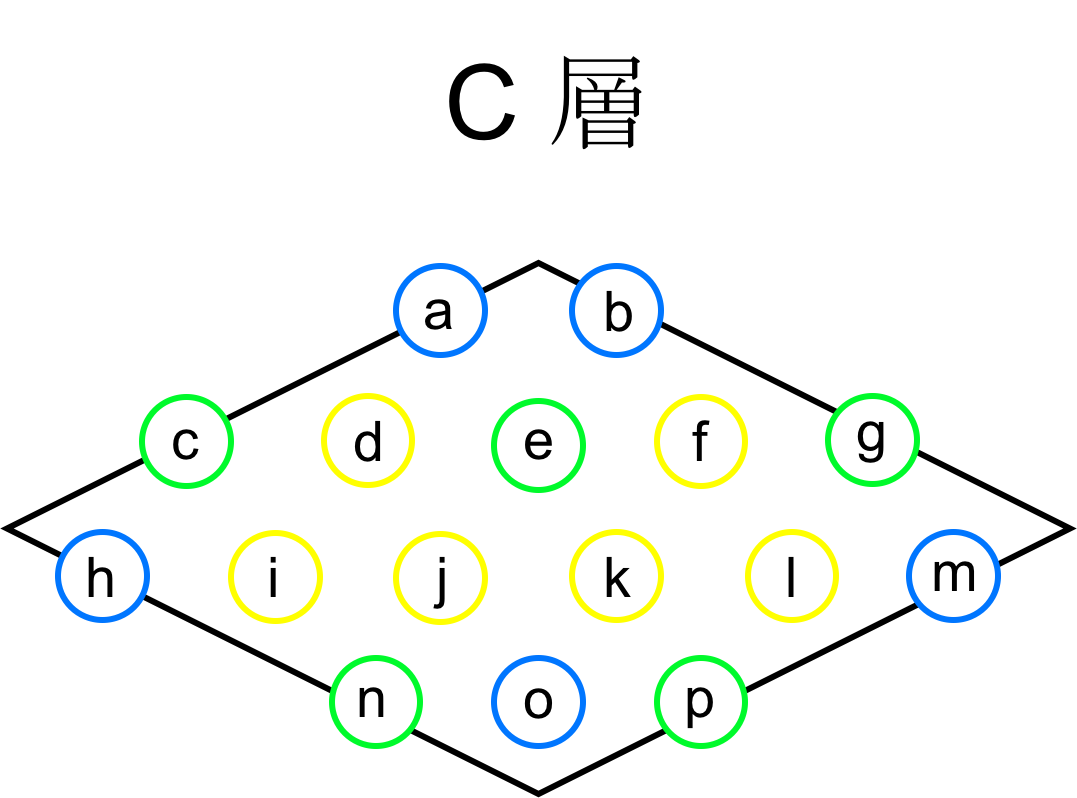
\includegraphics[width=80mm]{../method/Clayer.png}
        \label{default}
      \end{minipage}
    \end{tabular}
    \begin{center}
		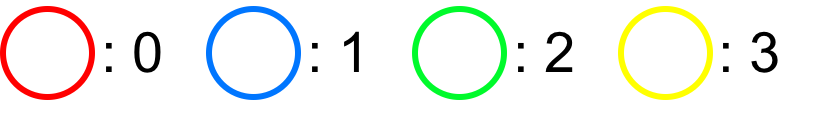
\includegraphics[width=50mm]{../method/AClayer.png}
		\caption{配置パターンの模式図.}
		\label{default}
	\end{center}
  \end{figure}




